\documentclass[tikz,border=3pt]{standalone}
\usepackage{xcolor}
\usetikzlibrary{arrows.meta,positioning}
\definecolor{ink}{HTML}{25343C}
\definecolor{muted}{HTML}{667781}
\definecolor{orange}{HTML}{E58A36}
\definecolor{orangebg}{HTML}{FFF5E9}
\definecolor{teal}{HTML}{218A81}
\definecolor{tealbg}{HTML}{EEF9F6}
\definecolor{coral}{HTML}{D9585C}
\definecolor{coralbg}{HTML}{FFF0F1}
\definecolor{violet}{HTML}{765AB5}
\definecolor{violetbg}{HTML}{F4F0FC}
\definecolor{blue}{HTML}{3E78C5}
\definecolor{bluebg}{HTML}{EEF4FE}
\definecolor{green}{HTML}{4B9969}
\definecolor{greenbg}{HTML}{EEF9F1}
\begin{document}
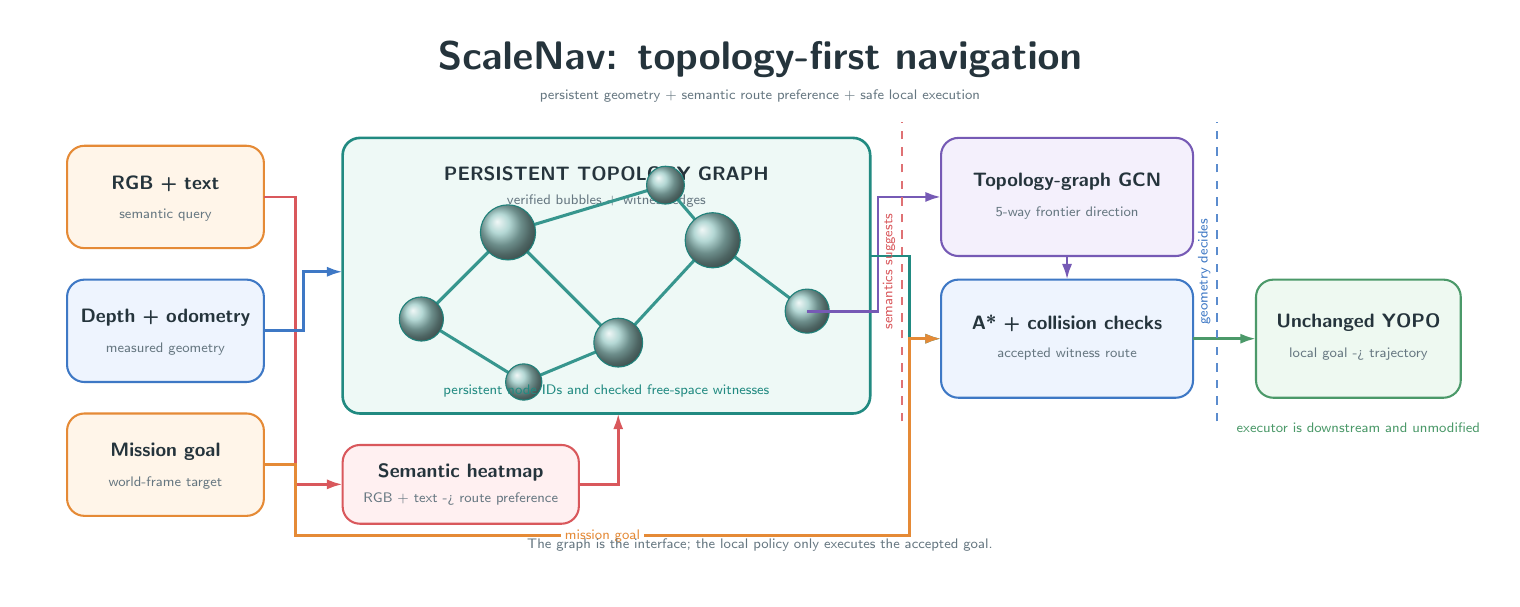
\begin{tikzpicture}[
 x=1mm,y=1mm,font=\sffamily,
 title/.style={font=\sffamily\bfseries\fontsize{13.5}{15.5}\selectfont,text=ink},
 head/.style={font=\sffamily\bfseries\fontsize{7.3}{8.4}\selectfont,text=ink,align=center},
 body/.style={font=\sffamily\fontsize{5.3}{6.2}\selectfont,text=muted,align=center},
 card/.style={rounded corners=2.2mm,line width=.75pt,align=center},
 flow/.style={-{Latex[length=2mm,width=1.3mm]},line width=1pt}
]
\fill[white] (-3,-3) rectangle (183,67);
\node[title] at (90,63) {ScaleNav: topology-first navigation};
\node[body] at (90,58.3) {persistent geometry  +  semantic route preference  +  safe local execution};

% Inputs.
\filldraw[card,draw=orange,fill=orangebg] (2,39) rectangle (27,52);
\node[head] at (14.5,47.2) {RGB + text};
\node[body] at (14.5,43.2) {semantic query};
\filldraw[card,draw=blue,fill=bluebg] (2,22) rectangle (27,35);
\node[head] at (14.5,30.2) {Depth + odometry};
\node[body] at (14.5,26.2) {measured geometry};
\filldraw[card,draw=orange,fill=orangebg] (2,5) rectangle (27,18);
\node[head] at (14.5,13.2) {Mission goal};
\node[body] at (14.5,9.2) {world-frame target};

% Central persistent graph.
\filldraw[card,draw=teal,fill=tealbg,line width=.95pt] (37,18) rectangle (104,53);
\node[head] at (70.5,48.5) {PERSISTENT TOPOLOGY GRAPH};
\node[body] at (70.5,45) {verified bubbles + witness edges};
\draw[teal!90,line width=1.1pt] (47,30)--(58,41)--(72,27)--(84,40)--(96,31);
\draw[teal!90,line width=1.1pt] (58,41)--(78,47)--(84,40);
\draw[teal!90,line width=1.1pt] (47,30)--(60,22)--(72,27);
\foreach \x/\y/\r in {47/30/2.8,58/41/3.5,72/27/3.1,84/40/3.5,96/31/2.8,78/47/2.4,60/22/2.3} {
  \shade[ball color=teal!45!white] (\x,\y) circle (\r mm);
  \draw[teal!90!ink,line width=.4pt] (\x,\y) circle (\r mm);
}
\node[body,text=teal] at (70.5,20.8) {persistent node IDs and checked free-space witnesses};

% Semantic fusion branch.
\filldraw[card,draw=coral,fill=coralbg] (37,4) rectangle (67,14);
\node[head] at (52,10.5) {Semantic heatmap};
\node[body] at (52,7.1) {RGB + text  ->  route preference};
\draw[flow,draw=coral] (27,45.5)--(31,45.5)--(31,9)--(37,9);
\draw[flow,draw=coral] (67,9)--(72,9)--(72,18);
\draw[flow,draw=blue] (27,28.5)--(32,28.5)--(32,36)--(37,36);

% Graph policy and route planning.
\filldraw[card,draw=violet,fill=violetbg] (113,38) rectangle (145,53);
\node[head] at (129,47.5) {Topology-graph GCN};
\node[body] at (129,43.5) {5-way frontier direction};
\filldraw[card,draw=blue,fill=bluebg] (113,20) rectangle (145,35);
\node[head] at (129,29.5) {A* + collision checks};
\node[body] at (129,25.5) {accepted witness route};
\draw[flow,draw=violet] (96,31)--(105,31)--(105,45.5)--(113,45.5);
\draw[flow,draw=teal] (104,38)--(109,38)--(109,27.5)--(113,27.5);
\draw[flow,draw=violet] (129,38)--(129,35);

% Executor.
\filldraw[card,draw=green,fill=greenbg] (153,20) rectangle (179,35);
\node[head] at (166,29.5) {Unchanged YOPO};
\node[body] at (166,25.5) {local goal -> trajectory};
\draw[flow,draw=green] (145,27.5)--(153,27.5);
\node[body,text=green] at (166,16.2) {executor is downstream and unmodified};

% Mission goal enters route planning; it is never sent directly to the executor.
\draw[flow,draw=orange] (27,11.5)--(31,11.5)--(31,2.5)--(109,2.5)--(109,27.5)--(113,27.5);
\node[body,text=orange,fill=white,inner sep=.5mm] at (70,2.5) {mission goal};

% Minimal safety boundary.
\draw[coral!85,dashed,line width=.7pt] (108,17)--(108,55);
\node[body,text=coral,rotate=90] at (106.4,36) {semantics suggests};
\draw[blue!85,dashed,line width=.7pt] (148,17)--(148,55);
\node[body,text=blue,rotate=90] at (146.4,36) {geometry decides};
\node[body] at (90,1.3) {The graph is the interface; the local policy only executes the accepted goal.};
\end{tikzpicture}
\end{document}
